\begin{minipage}[c]{\textwidth}
\advance\leftskip-2.5cm
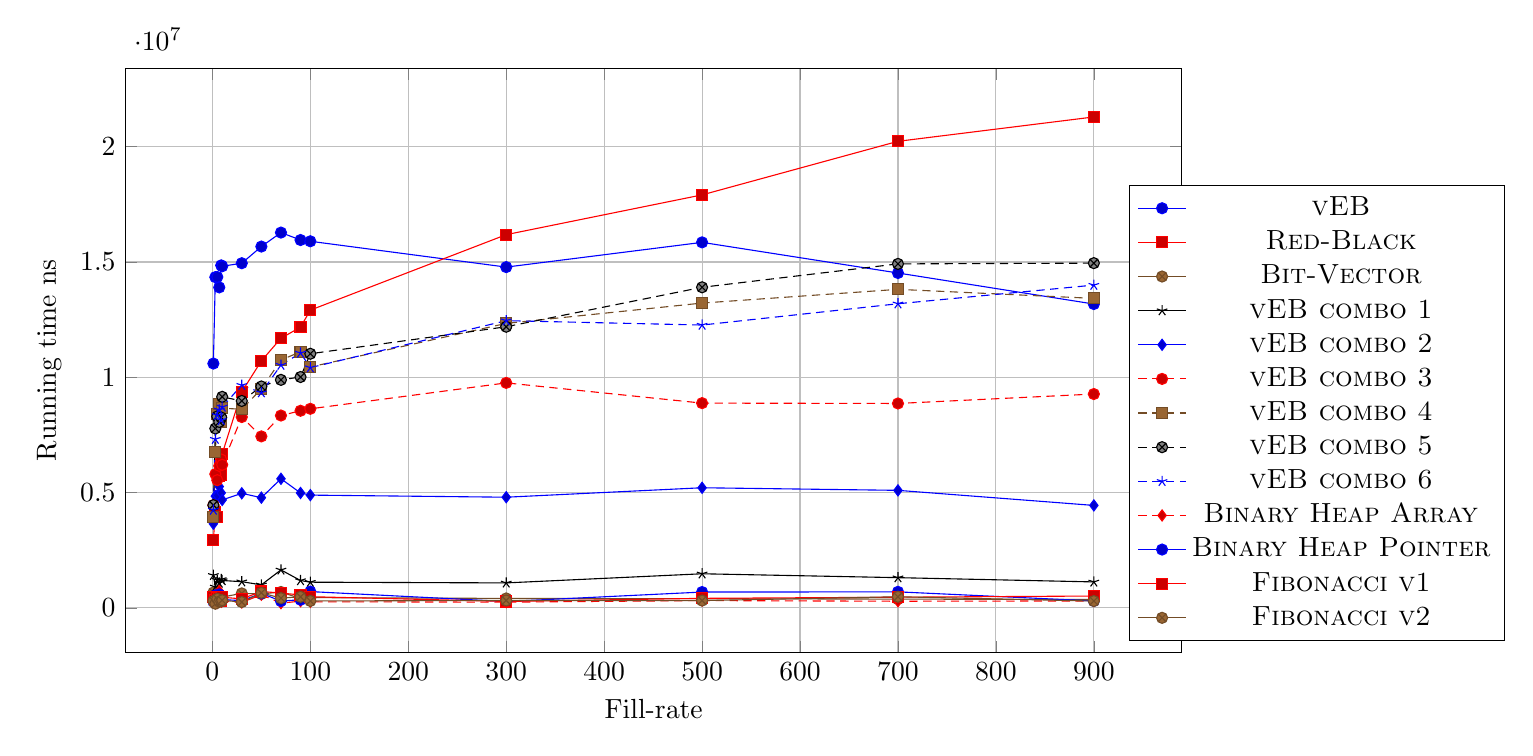
\begin{tikzpicture}
        \begin{axis}[
            xlabel = Fill-rate,
            ylabel = Running time ns,
            height=9cm,
            width=15cm,
            grid=major,
            legend style={
            at={(0.95,0.8)},
            anchor=north west}]            
            legend pos=center west
    	]
    		
    		
    	\addplot coordinates {
(1,10594290)
(3,14341481)
(5,14347849)
(7,13897463)
(9,14851770)
(10,14813042)
(30,14945554)
(50,15667620)
(70,16274540)
(90,15951603)
(100,15897028)
(300,14777090)
(500,15849857)
(700,14521126)
(900,13174934)

    	};
        
    	\addlegendentry{\textsc{vEB}}

                \addplot coordinates {
(1,2946080)
(3,4139732)
(5,3935356)
(7,5721888)
(9,5744907)
(10,6677458)
(30,9366338)
(50,10708854)
(70,11691602)
(90,12172518)
(100,12910732)
(300,16184309)
(500,17909156)
(700,20232455)
(900,21289179)

    	};
        
    	\addlegendentry{\textsc{Red-Black}}

        \addplot coordinates {
(1,662805)
(3,439108)
(5,410337)
(7,424816)
(9,415643)
(10,466015)
(30,625763)
(50,601039)
(70,688058)
(90,400927)
(100,442912)
(300,407291)
(500,395255)
(700,377521)
(900,362217)

    	};
        
    	\addlegendentry{\textsc{Bit-Vector}}

        \addplot coordinates {
(1,1411611)
(3,903893)
(5,1197517)
(7,1075567)
(9,1231658)
(10,1185278)
(30,1132512)
(50,996593)
(70,1643994)
(90,1184076)
(100,1111891)
(300,1080472)
(500,1476362)
(700,1308084)
(900,1123248)

    	};
        
    	\addlegendentry{\textsc{vEB combo 1}}

        \addplot coordinates {
(1,3646405)
(3,4842905)
(5,4875403)
(7,5257376)
(9,4985112)
(10,4680443)
(30,4965873)
(50,4776142)
(70,5596808)
(90,4981562)
(100,4888138)
(300,4797253)
(500,5207163)
(700,5094975)
(900,4441310)

    	};
        
    	\addlegendentry{\textsc{vEB combo 2}}

        \addplot coordinates {
(1,4453055)
(3,5800057)
(5,5536270)
(7,6156904)
(9,6433462)
(10,6203890)
(30,8274155)
(50,7435298)
(70,8339659)
(90,8546644)
(100,8631109)
(300,9755207)
(500,8877829)
(700,8862837)
(900,9271803)

    	};
        
    	\addlegendentry{\textsc{vEB combo 3}}
		
        \addplot coordinates {
(1,3929928)
(3,6763380)
(5,8406370)
(7,8853837)
(9,8078463)
(10,8658029)
(30,8611522)
(50,9496998)
(70,10743365)
(90,11106502)
(100,10445735)
(300,12335605)
(500,13217234)
(700,13812615)
(900,13420244)

    	};
        
    	\addlegendentry{\textsc{vEB combo 4}}
		
        \addplot coordinates {
(1,4453544)
(3,7778047)
(5,8301902)
(7,8062266)
(9,8256673)
(10,9150457)
(30,8971717)
(50,9600746)
(70,9886461)
(90,10009940)
(100,11019309)
(300,12190062)
(500,13901319)
(700,14916431)
(900,14949103)

    	};
        
    	\addlegendentry{\textsc{vEB combo 5}}

        \addplot coordinates {
(1,4241723)
(3,7313558)
(5,8351169)
(7,8584518)
(9,8136607)
(10,8711475)
(30,9654431)
(50,9331158)
(70,10527132)
(90,11051669)
(100,10416557)
(300,12454464)
(500,12264743)
(700,13187775)
(900,13995990)

    	};
        
    	\addlegendentry{\textsc{vEB combo 6}}
		
        \addplot coordinates {
(1,321315)
(3,292556)
(5,215121)
(7,730467)
(9,262790)
(10,293748)
(30,231534)
(50,568553)
(70,202894)
(90,289182)
(100,261174)
(300,246311)
(500,313787)
(700,286012)
(900,298242)

    	};
        
    	\addlegendentry{\textsc{Binary Heap Array}}

        \addplot coordinates {
(1,267939)
(3,541067)
(5,280841)
(7,578232)
(9,351427)
(10,357939)
(30,311950)
(50,625101)
(70,294468)
(90,349736)
(100,703284)
(300,273574)
(500,683813)
(700,692211)
(900,298164)

    	};
        
    	\addlegendentry{\textsc{Binary Heap Pointer}}

        \addplot coordinates {
(1,456146)
(3,337502)
(5,444872)
(7,446978)
(9,319553)
(10,457759)
(30,388491)
(50,707796)
(70,640301)
(90,558117)
(100,482365)
(300,276934)
(500,410785)
(700,460260)
(900,511763)

    	};
        
    	\addlegendentry{\textsc{Fibonacci v1}}

        \addplot coordinates {
(1,294266)
(3,177667)
(5,393286)
(7,268096)
(9,281338)
(10,328198)
(30,249705)
(50,649602)
(70,420986)
(90,477994)
(100,297104)
(300,318921)
(500,313547)
(700,479806)
(900,293045)

    	};
        
    	\addlegendentry{\textsc{Fibonacci v2}}

        \end{axis}

    \end{tikzpicture}
    \captionof{figure}{TITEL}
    \label{fig:sample_figure}
\end{minipage}